\section{Approach overview}

We present in this section an overview for PAMELA approach.

\subsection{Model serialization in source code}

We advocate for a strong coupling between model and source-code, to give architects and developers a way to both interact during the whole development cycle. PAMELA is an annotation-based Java modeling framework providing a smooth integration between model and code, without code generation nor externalized model serialization. The idea is to avoid separation between modeling and code to facilitate consistency management and avoid round-tripping issues.

To do so, we argue that source code is the right artefact to encode the model with metadata information stored in tagged code. This requires an annotation-enabled language. Such language supports the attribute-oriented programming if its grammar allows adding custom declarative tags to annotate standard program elements. Java programming language from version 1.5 is a good candidate with the support of annotations.

\begin{figure}
    \centering
    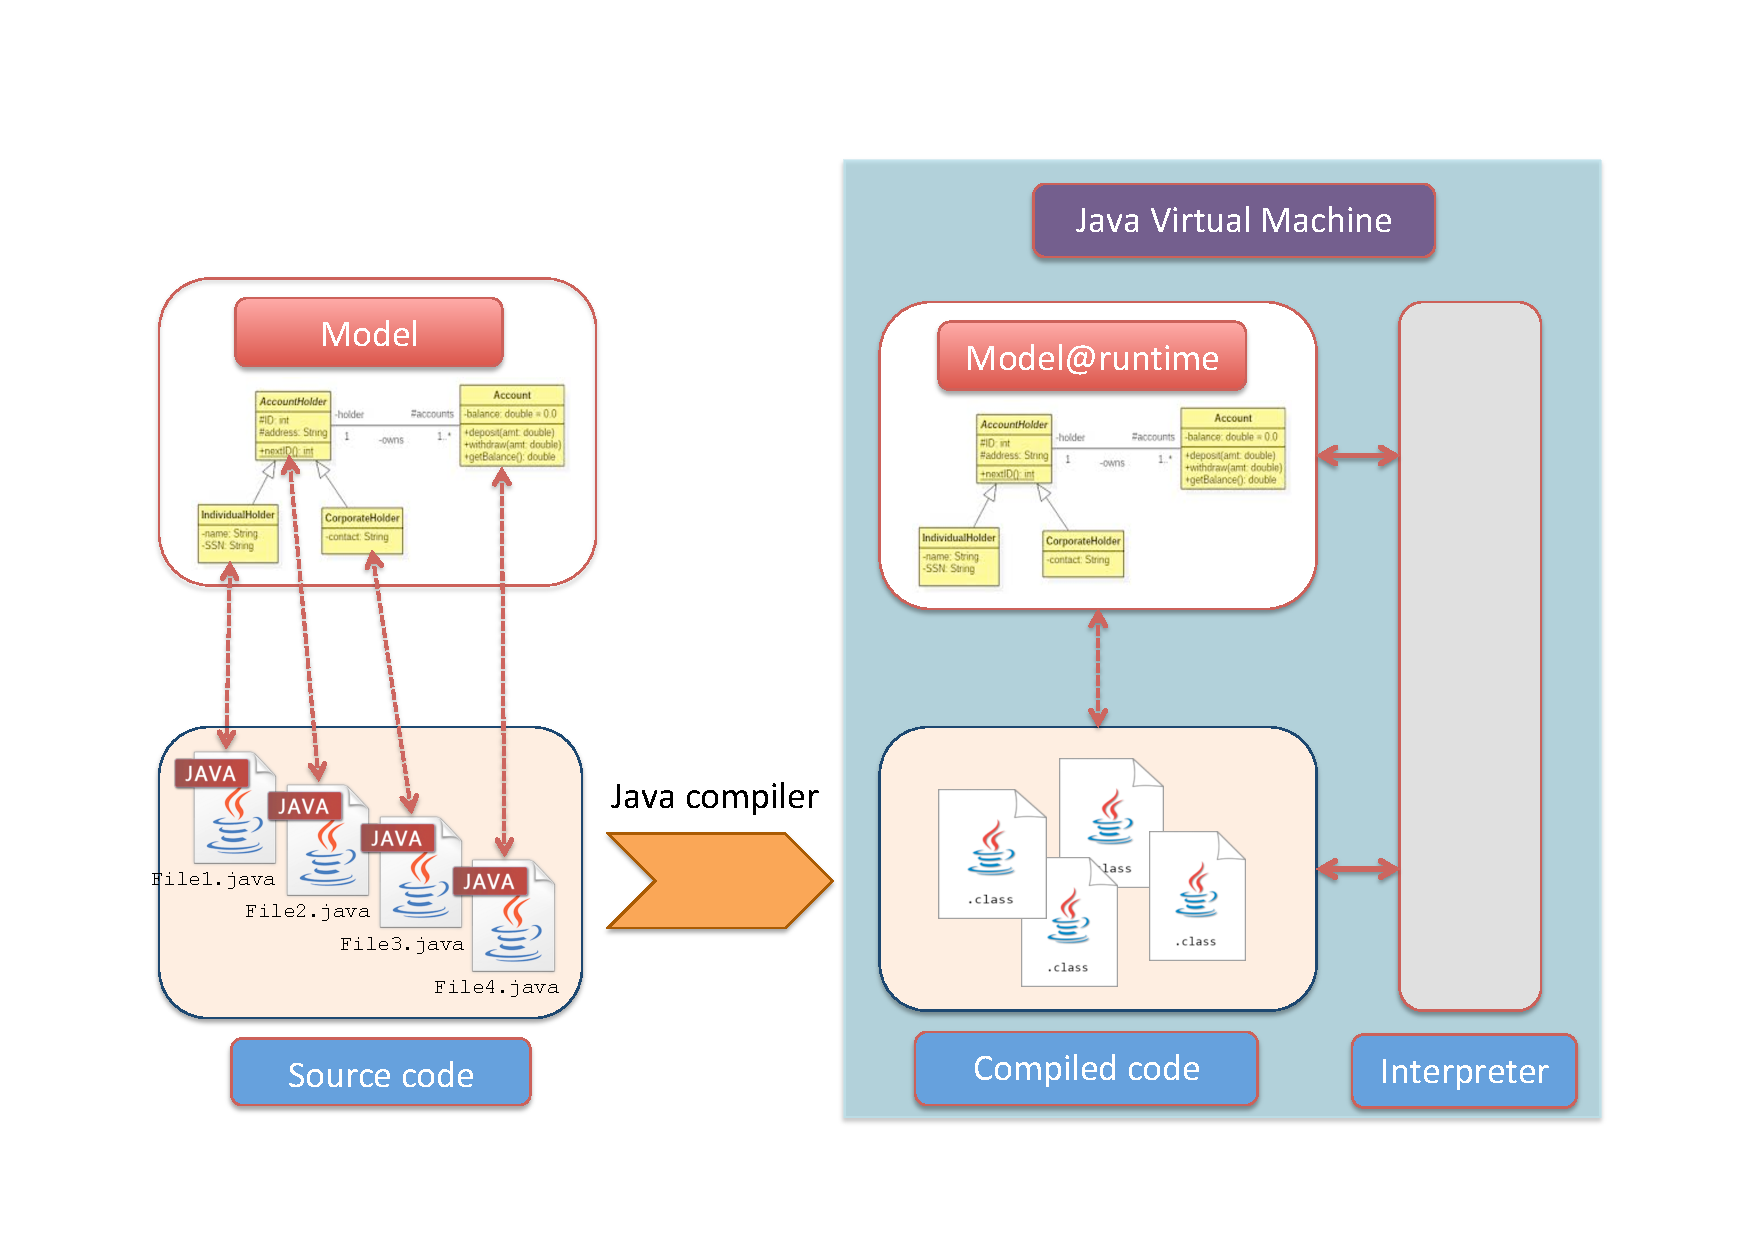
\includegraphics[width=1.0 \columnwidth]{PamelaVision.pdf}
    \caption{PAMELA approach for modelling}
    \label{fig:PamelaVision}
\end{figure}

Figure \ref{fig:PamelaVision} shows PAMELA approach for storing model in source code. The model is inlined in many source code files, with a set of annotations covering PAMELA metamodel as presented in the next subsection.

\subsection{PAMELA use process}

Coupling model and code into the same artefact open new ways of programming. The classical way relies on \emph{programmers} that produce code reusing pre-existing modeling concepts. These concepts are implemented by \emph{modelers} that provides the right annotations the programmers use. This is, for instance, the process followed by JEE developers reusing JEE specific annotations. The evolution rhythm between models and code is low. This programming way is still possible with PAMELA, but we allow the ability to reach a high evolution rhythm when the programmer becomes also the modeler. In fact, when a pattern, an abstraction, a generalization is identified by the programmer, s/he can use PAMELA to develop and capitalize on this abstraction by increasing PAMELA metamodel. 
The developed metamodels are implemented by annotations that relies on Java/JVM entities and mechanisms. They include consistency checking that constrains their use and help the programmer. We have experimented their use with setter/getter to define POJO entities, with traits to implement multiple inheritance or roles and rules to set security rules on classes.

Our experience shows that introducing and reusing new concepts (1) reduce the size of the code, (2) reduce the risk of errors and (3) improve the code structure. The cycle of development between the model and the code can then be drastically reduced, leading to what we call \emph{continuous modeling}.

The code size is reduced because abstractions factorized the recognize pattern and the previous code is replaced by the use of the abstraction at the right place. This also reduces the risk since the previous code is now generated by the PAMELA framework with all the required checks. And finally, the code structure is improved since it matches the way the programmer conceptualizes (models) her/his code. 

\subsection{PAMELA metamodel}

PAMELA metamodel is presented in figure \ref{fig:PamelaMetaModel}.
This metamodel is classical and reflects a common class diagram vision such as in UML. 

\begin{figure}
    \centering
    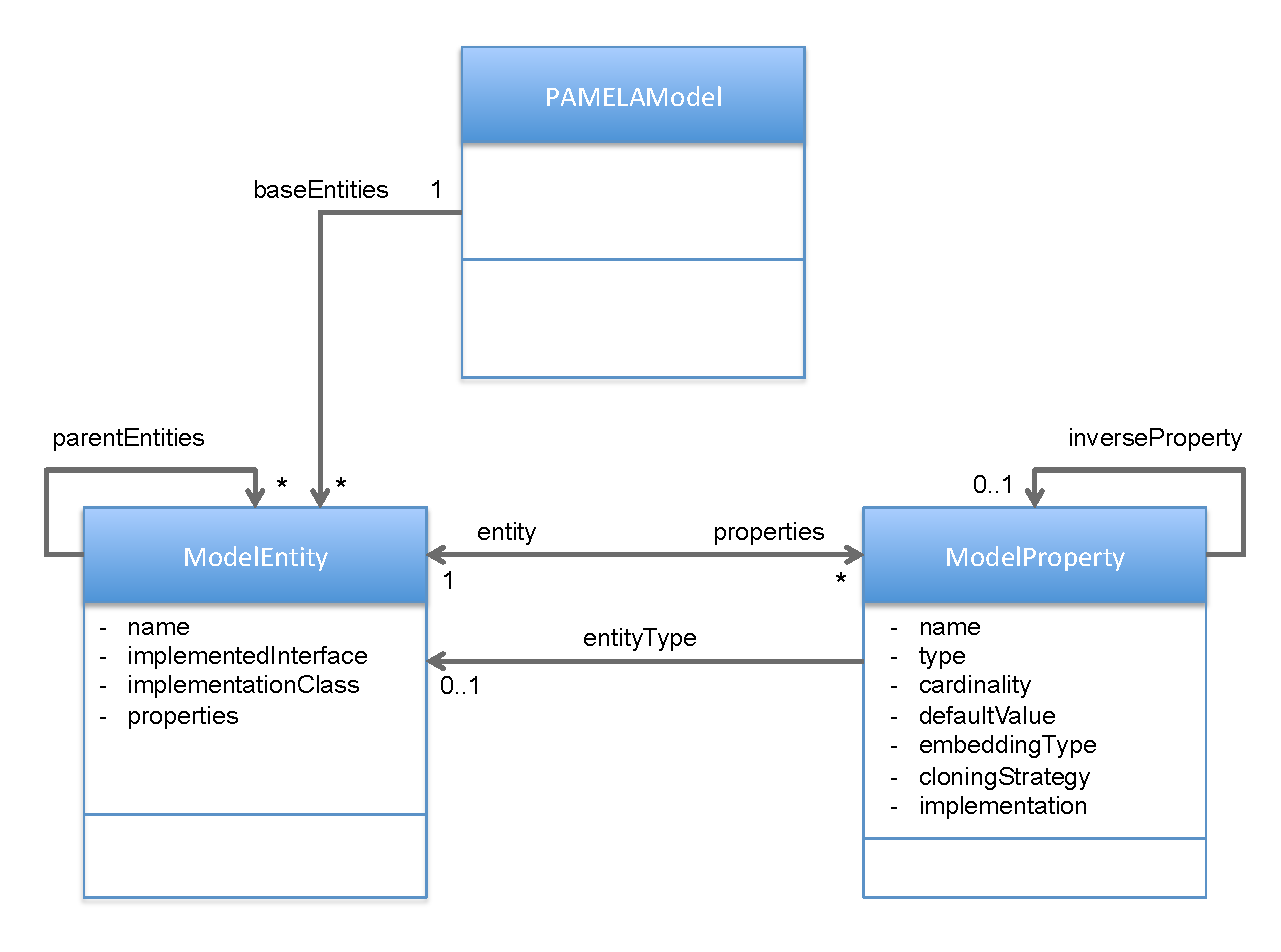
\includegraphics[width=1.0 \columnwidth]{PamelaMetaModel.pdf}
    \caption{PAMELA metamodel}
    \label{fig:PamelaMetaModel}
\end{figure}

\subsubsection{PAMELAModel}

A \texttt{PAMELAModel} is defined as a set of references to \texttt{ModelEntity}. 

\subsubsection{ModelEntity}

A \texttt{ModelEntity} reflects a concept and is encoded in a java \texttt{interface}. PAMELA metamodel allows multiple inheritance: thus \texttt{ModelEntity} may define a set of parent entities. A \texttt{ModelEntity} also defines some properties, encoded as \texttt{ModelProperty}. Note that reification of \texttt{ModelEntity} is performed in a java \texttt{interface} (and not a class), which only defines API whithout any implementation for methods. A partially implemented \texttt{abstract} java texttt{class} may be defined as partial base implementation (conform to implemented interface).

\subsubsection{ModelProperty}

A \texttt{ModelProperty} is identified by a name, a cardinality (simple or multiple) and a type, which can be a reference to another \texttt{ModelEntity}, or a Java type (a primitive or an arbitrary complex Java type). Depending on its cardinality, a \texttt{ModelProperty} is bound to a set of methods reflecting use of property.
\begin{itemize}
    \item A \emph{read-only single property} will define read-access of its value using a \emph{getter} (a java method defined in java interface taking no argument and returning desired value).
    \item A \emph{read-write single property} will define a \emph{getter} and a \emph{setter} (a java method taking value to be set as unique argument)
    \item A \emph{read-write multiple property} will define a \emph{getter}, a \emph{adder} (a java method taking value to be added as unique argument), a \emph{remover} (a java method taking value to be removed as unique argument), and may define additional methods for extended features such as reindexing for example.
\end{itemize}

A strong interest of the approach is that the model is encoded in java, and must be compiled. It forces the java compiler to perform required checks for a PAMELA model encoded in a strong typed program. Execution semantics of model is fully compatible with Java semantics. Many validation rules are automatically performed through classical java compilation, independently of underlying PAMELA execution semantics.

\subsection{A basic example}

The following code listing represents a very basic model with two entities \emph{Book} and \emph{Library}. Entity \emph{Book} defines two read-write single properties \emph{title} and \emph{ISBN} with single cardinality and with \texttt{String} type. Entity \emph{Book} also define a constructor with initial \emph{title} value. Entity \emph{Library} defines a read-write multiple properties \emph{books} referencing \emph{Book} instances. Note that this code is sufficient to execute the model, while no line of code is required (only java interface and API methods are declared here). 

%\begin{figure}
%    \centering
\begin{lstlisting}[language=Java,basicstyle=\ttfamily\footnotesize]
@ModelEntity
public interface Book 
  extends AccessibleProxyObject {
  @Initializer
  public Book init(@Parameter("title") 
    String aTitle);
  @Getter("title")
  public String getTitle();
  @Setter("title")
  public void setTitle(String aTitle);
  @Getter("ISBN")
  public String getISBN();
  @Setter("ISBN")
  public void setISBN(String value);
}

@ModelEntity
public interface Library
  extends AccessibleProxyObject {
  @Getter(value = "books", 
    cardinality = Cardinality.LIST)
  public List<Book> getBooks();
  @Adder("books")
  public void addToBooks(Book aBook);
  @Remover("books")
  public void removeFromBooks(Book aBook);
  @Reindexer("books")
  public void moveBookToIndex(Book aBook, 
    int index);
  @Finder(collection = "books",
    attribute = "title")
  public Book getBook(String title);
}
\end{lstlisting}
 %   \caption{A basic PAMELA model with two entities \texttt{Library} and \texttt{Book}}
 %   \label{fig:ABasicPamelaModel}
%\end{figure}

Execution of this model may be performed using following simple lines of code.

%\begin{figure}
%    \centering
\begin{lstlisting}[language=Java,basicstyle=\ttfamily\footnotesize]
// Instantiate the meta-model
// by computing the closure of concepts graph
ModelContext modelContext = ModelContextLibrary
  .getModelContext(Library.class);
// Instantiate the factory
ModelFactory factory 
  = new ModelFactory(modelContext);
// Instantiate a Library
Library myLibrary 
  = factory.newInstance(Library.class);
myLibrary.setName("My library");
// Instantiate some Books
Book myFirstBook = factory.newInstance(
  Book.class, "Lord of the ring");
Book anOtherBook = factory.newInstance(
  Book.class, "Holy bible");
myLibrary.addToBooks(myFirstBook);
myLibrary.addToBooks(anOtherBook);
\end{lstlisting}
 %   \caption{Executing a PAMELA model}
 %   \label{fig:ExecutingPamelaModel}
%\end{figure}

The first line of code instantiates a \texttt{ModelContext} by introspecting and computing the closure of concepts graph obtained while starting from \texttt{Library} entity and following \texttt{parentEntities} and \texttt{properties} relationships. This call builds at runtime a \emph{PAMELAModel}, while dynamically following links reflected by compiled byte-code. A factory \texttt{ModelFactory} is then instantiated using that \texttt{ModelContext}, allowing to instantiate \emph{Library} and \emph{Book} instances.

\subsection{Handling custom code}

A major challenge to be addressed by MDE (Model-Driven Engineering) approaches is the ability to integrate custom implementation to a base of code derived from a formal model. The major drawback is the way back (round-tripping).

PAMELA frameworks provides an elegant way to do it, while using common extension points such as inheritance, as offered by java language. Custom implementations should be declared in java classes, this or those classes declared as partial implementation(s) of related \emph{ModelEntity}. 

The following example shows how to integrate custom code to the fully interpreted \emph{Book} entity described above. The partial custom implementation is offered by a partial class (note the \texttt{abstract} keyword), declared in annotation header of model entity. Custom implementations are defined using classical java implementation/overrides scheme. Here we define implementation of \texttt{read()} method, which has no annotation (and thus unable to be processed by PAMELA framework), and also implementation of a custom getter for \emph{title}, returning a default value when no value is defined for that property. Note that this implementation references default interpretated implementation (call to \texttt{performSuperGetter(String)} method).

%\begin{figure}
%    \centering
\begin{lstlisting}[language=Java,basicstyle=\ttfamily\footnotesize]
@ModelEntity
@ImplementationClass(BookImpl.class)
public interface Book 
  extends AccessibleProxyObject {
  static final String TITLE = "title";
  @Getter(TITLE)
  String getTitle();
  // ... title property declarations ...
  void read();
}
// Provides a partial implementation for Book
public static abstract class BookImpl 
  implements Book {
  @Override
  public String getTitle() {
    String title = performSuperGetter(TITLE);
    if (title == null) {
      return "This book has no title";
    }
    return title;
  }
  @Override
    public void read() {
      // do the job
    }
}
\end{lstlisting}
 %   \caption{Executing a PAMELA model}
 %   \label{fig:ExecutingPamelaModel}
%\end{figure}

As said previously, PAMELA framework supports multiple inheritance. In this context, it is possible to provide multiple partial classes as implementation for a given \emph{ModelEntity}. To do so, we use abstract inner classes tagged with \texttt{@Implementation}, and the composition is made at run-time.

\subsection{Run-time considerations}

Resulting model execution is a combination of:
\begin{itemize}
    \item plain java byte-code, as the result of the basic compilation of source code,
    \item and an embedded PAMELA interpreter, executing semantics reflected by \emph{ModelEntity} and \emph{ModelProperty} declarations.
\end{itemize}
 
This composition offers many benefits: 
\begin{itemize}
    \item Strong coupling between model and code
    \item Strong typing is kept, and required checks are performed by the java compiler
    \item PAMELA framework provides interpretation of model@runtime
    \item No need to generate POJO (plain old java objects), as their execution follow the standard semantics (less code, less bugs)
    \item Custom implementation are provided if needed, using classical java extension points
    \item It offers a way to intercept method calls and instrument the code
\end{itemize}

From a technical point of view, PAMELA implementation uses \emph{javassist} reflection library, providing \texttt{MethodHandler} mechanism, which is a way to override the java dynamic binding. Invoking a method on an object which is part of a PAMELA model, caused the real implementation to be called when existing (more precisely dispatch code execution between all provided implementations), or the required interpretation according to underlying model to be executed. This provides also an extension point allowing to instrument the code, which is used for other features such as undo/redo stack management, and assertion checking at run-time (support for Design by Contract, aka JML).
% TODO: trouver des références pour ca

PAMELA framework is a 100\% pure java (> 1.5), compilable by a classical java compiler and executable in a classical Java Virtual Machine.

% Rajouter un paragraphe sur le fait que PAMELA est une implementation du MOP (meta object protocol) ?

\subsection{Common PAMELA annotations}

Here is a non-exhaustive list of the most common java annotations reflecting PAMELA metamodel.

\begin{itemize}
    \item \texttt{@ModelEntity}: tag annotating \texttt{interface} as \emph{ModelEntity}. May declares an abstract entity.
    \item \texttt{@ImplementationClass}: tag annotating \emph{ModelEntity} \texttt{interface} and precising abstract java \texttt{class} to be used as base implementation.
    \item \texttt{@Implementation}: tag annotating a partial implementation (abstract inner \texttt{class} defined in implemented \texttt{interface}), and used in the context of multiple inheritance.
    \item \texttt{@Getter(String)}: tag annotating method as unique getter for implicit \emph{ModelProperty} whose identifier is the declared String value. May also declares cardinality, enventual inverse property, default value and some other features.
    \item \texttt{@Setter(String)}: tag annotating method as unique setter for implicit \emph{ModelProperty} whose identifier is the declared String value.
    \item \texttt{@Adder(String)}: tag annotating method as unique adder for implicit multiple cardinality \emph{ModelProperty} whose identifier is the declared String value.
    \item \texttt{@Remover(String)}: tag annotating method as unique remover for implicit multiple cardinality \emph{ModelProperty} whose identifier is the declared String value.
    \item \texttt{@Reindexer(String)}: tag annotating method as unique reindexer for implicit multiple cardinality \emph{ModelProperty} whose identifier is the declared String value.
    \item \texttt{@Initializer}: tag annotating a method used as a constructor for related \emph{ModelEntity}
   \item \texttt{@Deleter}: tag annotating a method used as explicit destructor for related \emph{ModelEntity}
    \item \texttt{@Finder(String,String)}: tag annotating method as a fetching request for a given \emph{ModelProperty} with a given attribute
    \item \texttt{@CloningStrategy}: allows to customize cloning strategy for a given \emph{ModelProperty}
    \item \texttt{@Embedded}: allows to declare a given \emph{ModelProperty} as embedded according to PAMELA semantics
    \item \texttt{@Imports} and \texttt{@Imports}: allows to declare some entities to be included in infered metamodel while \texttt{ModelContext} computation.
    \item \texttt{@XMLElement} and \texttt{@XMLAttribute}: used to specify XML serialization for PAMELA instances
    
\end{itemize}



